
\documentclass{article}
\usepackage{graphicx}
\usepackage{tikz}


\begin{document}


%%%%%%%%%%%%%%%%%%%%%%%%%%%%%%%%%%%%%%%%%%%%%%%%%%%%%%%%%
\definecolor{bgcolor}{rgb}{0.98, 0.98, 1.0}
\newenvironment{tikzbox}
{\begin{tikzpicture}
    \node[fill=bgcolor,rounded corners=1em,draw=black,minimum width=0.9\linewidth]}
  {;\end{tikzpicture}}

%%%%%%%%%%%%%%%%%%%%%%%%%%%%%%%%%%%%%%%%%%%%%%%%%%%%%%%%%


\begin{figure}[ht!]
  %\vspace{-1.0em}
\begin{center}
  \begin{tikzbox} {
  \begin{tikzpicture}[minimum width=0]
    \tikzstyle{label} = [node distance = 2cm,text=blue]
    \tikzstyle{mycoord} = [node distance = 0cm]
    \tikzstyle{block} = [node distance = 1.5cm,rounded corners=.00cm,
    inner sep=.1cm, fill=bgcolor, minimum height=2em,minimum width=7em]
     \node[block,name=obj1] {
\includegraphics[width=0.2\textwidth]{./baseball.jpg} };
     \node[block,xshift=3cm,name=obj2] {
\includegraphics[width=0.2\textwidth]{./sodaCan.jpg} };
     \node[block,xshift=6cm,name=obj3] {
\includegraphics[width=0.2\textwidth]{./cerealBox.jpg} };
     \node[block,xshift=9cm,name=obj4] {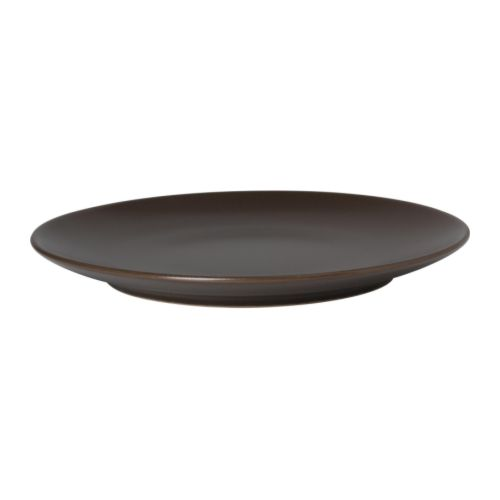
\includegraphics[width=0.2\textwidth]{./flatPlate.JPG} };
     \node[block,xshift=12cm,name=obj5] {
\includegraphics[width=0.2\textwidth]{./tuna.png} };
     \node[block,xshift=0cm,yshift=-4cm,name=sq1] {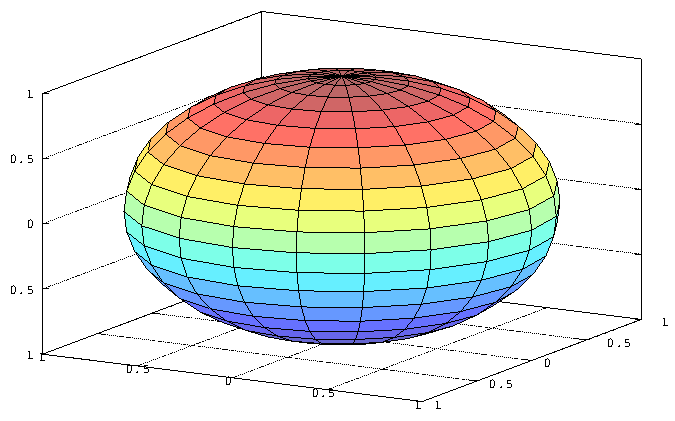
\includegraphics[width=0.2\textwidth]{./ball_fit.png} };
     \node[block,xshift=3cm,yshift=-4cm,name=sq2] {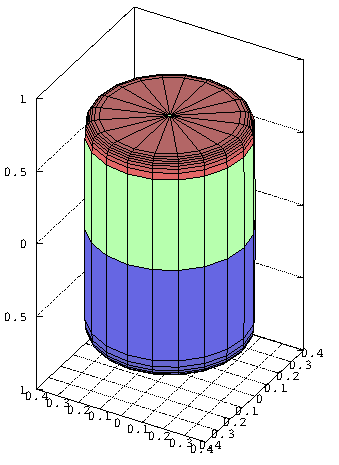
\includegraphics[width=0.2\textwidth]{./cylinder_fit.png} };
     \node[block,xshift=6cm,yshift=-4cm,name=sq3] {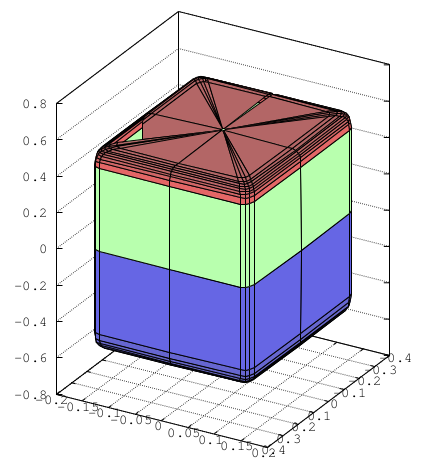
\includegraphics[width=0.2\textwidth]{./box_fit.png} };
     \node[block,xshift=9cm,yshift=-4cm,name=sq4] {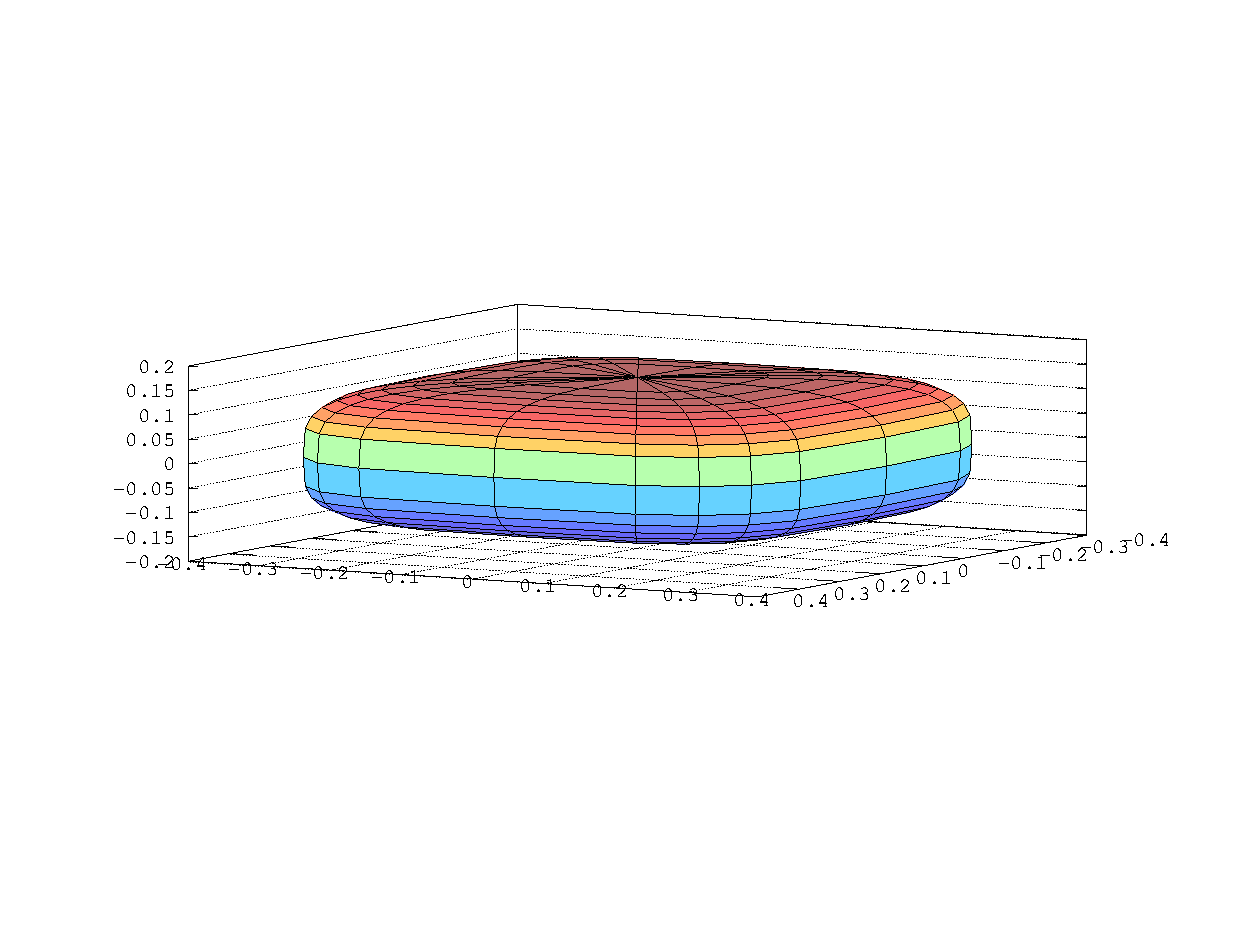
\includegraphics[width=0.2\textwidth]{./plate.eps} };
     \node[block,xshift=12cm,yshift=-4cm,name=sq5] {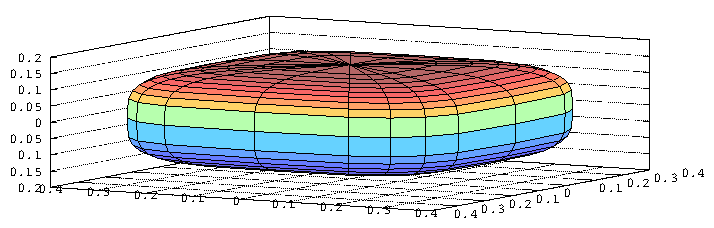
\includegraphics[width=0.2\textwidth]{./tunaCan_fit.png} };
     \node[label,below of=obj1]{Baseball};  
     \node[label,below of=obj2]{Soda can};
     \node[label,below of=obj3]{Cereal box};
     \node[label,below of=obj4]{IKEA plate};
     \node[label,below of=obj5]{Tuna};

     \node[label,below of=sq1]{$\epsilon_{1} = 1.0, \epsilon_{2}=1.0$};  
     \node[label,below of=sq2]{$\epsilon_{1} = 0.1, \epsilon_{2}=1.0$};
     \node[label,below of=sq3]{$\epsilon_{1} = 0.1, \epsilon_{2}=0.1$};
     \node[label,below of=sq4]{$\epsilon_{1} = 0.1, \epsilon_{2}=1.0$};
     \node[label,below of=sq5]{$\epsilon_{1} = 0.5, \epsilon_{2}=0.5$};


  \end{tikzpicture}
  }\end{tikzbox}
\caption{Why superquadrics are cool?}
\label{fig:coverImage}
\end{center}
\vspace{-2.0em}
\end{figure}


\end{document}